\chapter{\babLima}

\section{Analisis Pengujian Autentikasi  VxLang}
\subsection{Analisis Statis}
Analisis statis dilakukan untuk memahami mekanisme autentikasi aplikasi tanpa menjalankan kode. Alat yang digunakan dalam analisis ini adalah Ghidra, sebuah \f{software reverse engineering} yang menyediakan kemampuan \f{disassembly} dan \f{decompilation}. Tujuan utama dari analisis statis ini adalah untuk mengidentifikasi lokasi kode yang menangani proses autentikasi dan mencari potensi celah keamanan yang dapat dimanfaatkan untuk melewati proses tersebut.

\subsubsection{Analisis Aplikasi Non-Virtualized}
Pada aplikasi non-virtualized (konsol, Qt, dan ImGUI), proses analisis dimulai dengan mencari \f{string} yang relevan dengan autentikasi, seperti "Authentication Failed" atau \f{string} yang mungkin digunakan sebagai \f{username} atau \f{password}. Setelah \f{string} tersebut ditemukan, langkah selanjutnya adalah menelusuri referensi silang (\f{cross-references}) untuk melihat di mana \f{string} tersebut digunakan dalam kode program. Hal ini membantu dalam mengidentifikasi fungsi atau blok kode yang bertanggung jawab untuk menampilkan pesan kegagalan autentikasi, yang sering kali berdekatan dengan logika autentikasi itu sendiri.

Sebagai contoh, pada aplikasi \textit{app\_imgui}, analisis \f{disassembly} menggunakan Ghidra mengungkapkan potongan kode berikut:

\begin{listing}[H]
    \begin{minted}{asm}
; (Kode memuat input password ke register, misal RDI) ...

; (Kode memuat password hardcoded "rahman", misal ke alamat yg ditunjuk RDX)

LEA            RDX,[s_rahman_140110551]   = "rahman"
MOV            RCX,RDI
CALL           VCRUNTIME140.DLL::memcmp ; Bandingkan input & hardcoded pwd
CMP            RBX,0x6
TEST           EAX,EAX                  ; Cek hasil memcmp (EAX=0 jika sama)
JNZ            LAB_140003226            ; Lompat ke blok gagal jika EAX != 0

; (Blok kode jika autentikasi berhasil) 

LAB_140003226:  ; Label untuk blok gagal
LEA            RDX,[u_Authentication_Failed_1401104da] ; Load string "Auth Failed"
CALL           qword ptr [->USER32.DLL::MessageBoxW] ; Tampilkan pesan gagal

\end{minted}
\caption{Snippet Assembly: Perbandingan Password dan Lompatan Kondisional (Non-Virtualized)}
\label{lst:asm_static_nonvirt_snippet}
\end{listing}

Dalam konteks kode di atas, pemanggilan \code{memcmp} (di operasi \texttt{LEA}) membandingkan password yang dimasukkan pengguna dengan nilai "rahman" yang \textit{hardcoded} pada aplikasinya. Hasilnya diperiksa oleh \code{TEST EAX,EAX} (\texttt{140003216}). Jika password tidak sama, \code{EAX} tidak akan nol, dan instruksi \code{JNZ} (\texttt{140003218}, Jump if Not Zero) akan mengalihkan eksekusi ke \code{LAB\_140003226}, di mana pesan "Authentication Failed" ditampilkan. 

Untuk memvalidasi potensi celah keamanan, instruksi `JNZ LAB\_140003226` dapat diubah (\f{patched}) menjadi `JZ LAB\_140003226` atau instruksi lain yang akan selalu mengarahkan program untuk melewati blok kode yang menampilkan pesan kegagalan autentikasi. Dalam kasus ini, mengubah `JNZ` menjadi `JZ` (Jump if Zero) akan menyebabkan lompatan terjadi hanya jika hasil perbandingan adalah nol (yang menandakan autentikasi berhasil), sehingga secara efektif membalikkan logika dan memungkinkan akses tanpa otorisasi.

Lebih lanjut, analisis pada bagian \f{defined data} (.rdata) juga mengungkapkan adanya \f{string} `"seno"` dan `"rahman"`. Keberadaan \f{string-string} ini sangat mengindikasikan bahwa aplikasi menyimpan \f{username} dan \f{password} secara \f{hard-coded}. Praktik menyimpan kredensial secara langsung dalam kode program sangat berbahaya dari sudut pandang keamanan. String seperti ini mudah ditemukan melalui analisis statis, seperti yang telah dilakukan, sehingga penyerang dapat dengan mudah memperoleh informasi \f{username} dan \f{password} tanpa perlu melakukan \f{reverse engineering} yang mendalam atau menjalankan aplikasi. Dalam kasus ini, \f{username} `"seno"` dan \f{password} `"rahman"` yang ditemukan dalam \f{defined data} dapat dieksploitasi untuk melewati mekanisme autentikasi.

\begin{figure}
	\centering
	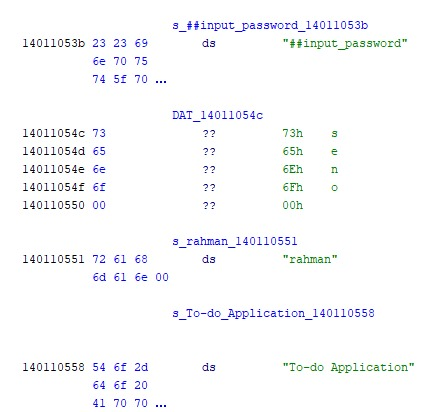
\includegraphics[width=0.45\textheight]
	{assets/pics/hardcoded_credentials.jpeg}
  \caption{\f{Hardcoded username \& password} pada \f{defined data}}
\end{figure}

Analisis serupa juga dilakukan pada aplikasi konsol dan Qt, di mana pola perbandingan string dan penggunaan instruksi kondisional untuk mengontrol alur program berdasarkan hasil autentikasi juga ditemukan dan dapat dimanipulasi dengan cara yang serupa untuk melewati proses autentikasi.

\subsubsection{Analisis Aplikasi Non-Virtualized (Versi Cloud)}
Untuk mengatasi risiko \f{hard-coded} username dan password, mekanisme autentikasi telah diubah menjadi berbasis \f{cloud}. Dalam versi \f{cloud} ini, aplikasi mengirimkan username dan password dalam format JSON ke server HTTP, yang kemudian melakukan verifikasi terhadap database PostgreSQL. Dengan perubahan ini, username dan password tidak lagi disimpan secara langsung di dalam aplikasi klien.

Meskipun kredensial tidak lagi \f{hard-coded}, analisis statis tetap relevan untuk memahami bagaimana aplikasi klien berinteraksi dengan server. Sebagai contoh, pada aplikasi \textit{console\_cloud}, analisis \f{disassembly} menggunakan Ghidra pada fungsi yang menangani autentikasi menunjukkan potongan kode berikut:

\begin{listing}[H]
    \begin{minted}[linenos=false]{asm}
; ... (Kode setelah fungsi send_login_request kembali, hasil mungkin di AL) ...
MOV      AL, byte ptr [RBP + local_69] ; Ambil hasil boolean?
TEST     AL, 0x1                       ; Cek bit 0 dari AL
JNZ      LAB_14000175d                 ; Lompat jika hasil != 0 (Sukses?)
JMP      LAB_14000178e                 ; Lompat jika hasil == 0 (Gagal?)

LAB_14000175d:  ; Blok kode jika sukses
; ... (Kode menampilkan "Authorized!") ...
jmp      LAB_END_AUTH_CHECK                       ; Lompat ke akhir

LAB_14000178e:  ; Blok kode jika gagal
; ... (Kode menampilkan "Not authorized") ...

\end{minted}
\caption{Snippet Assembly: Pemeriksaan Hasil Autentikasi Cloud (Non-Virtualized)}
\label{lst:asm_static_cloud_snippet}
\end{listing}

Pada kode di atas, instruksi \code{TEST AL, 0x1} kemungkinan memeriksa flag atau nilai boolean yang dikembalikan oleh fungsi autentikasi cloud (misalnya, 1 untuk sukses, 0 untuk gagal). Instruksi \code{JNZ LAB\_14000175d} kemudian mengarahkan alur eksekusi ke blok "Authorized!" jika hasil tes tidak nol (sukses), dan sebaliknya akan jatuh ke \code{JMP LAB\_14000178e} atau langsung mengeksekusi blok "Not authorized". Sama seperti kasus sebelumnya, instruksi \code{JNZ} ini dapat dimanipulasi (misal, diubah menjadi \code{JMP LAB\_14000175d} atau \code{NOP}) untuk memaksa alur ke blok sukses, meskipun server menolak autentikasi. Konteks assembly yang lebih lengkap dapat dilihat pada Lampiran \ref{app:kode_asm} (Kode \ref{lst:asm_static_cloud_full}).

Sama seperti pada kasus \f{hard-coded} sebelumnya, instruksi `JNZ LAB\_14000175d` dapat diubah menjadi `JZ LAB\_14000175d`. Dengan perubahan ini, program akan selalu melompat ke bagian yang menampilkan "Authorized!" tanpa perlu melakukan verifikasi yang sebenarnya dari server. Meskipun username dan password tidak lagi disimpan di dalam aplikasi, logika di sisi klien yang menentukan apakah autentikasi berhasil atau gagal masih dapat dimanipulasi.

Ini menunjukkan bahwa meskipun memindahkan logika autentikasi ke server dan menghindari \f{hard-coded credential} meningkatkan keamanan, sisi klien aplikasi masih dapat menjadi target untuk \f{reverse engineering}. Penyerang dapat memodifikasi aplikasi klien untuk selalu menganggap autentikasi berhasil, meskipun server mungkin menolak permintaan autentikasi. Oleh karena itu, keamanan menyeluruh memerlukan perlindungan tidak hanya pada kredensial tetapi juga pada logika bisnis aplikasi di sisi klien.

Analisis serupa juga dilakukan pada aplikasi konsol dan ImGUI versi \f{cloud}, di mana pola pemeriksaan kondisi dan jump kondisional yang menentukan status autentikasi juga ditemukan dan berpotensi untuk dimanipulasi.

\subsubsection{Analisis Aplikasi Virtualized}

Analisis statis pada aplikasi yang telah divirtualisasi menggunakan VxLang menunjukkan tingkat kesulitan yang jauh lebih tinggi dibandingkan versi non-virtualized. Observasi kualitatif sebelumnya diperkuat oleh data kuantitatif yang diperoleh dari ringkasan analisis Ghidra terhadap \f{executable} \code{app\_qt.exe} (asli) dan \code{app\_qt\_vm.exe} (virtualized), seperti yang dirangkum dalam Gambar \ref{fig:ghidra_summary_qt} dan \ref{fig:ghidra_summary_qt_vm}.

Beberapa temuan kuantitatif dan kualitatif signifikan adalah:

\begin{itemize}
    \item \bo{Hilangnya Informasi Struktural Fundamental:} Perbedaan paling mencolok adalah Ghidra melaporkan \textbf{0 instruksi} dan \textbf{0 fungsi} yang terdeteksi pada \code{app\_qt\_vm.exe}, dibandingkan dengan 9133 instruksi dan 678 fungsi pada \code{app\_qt.exe} (lihat Gambar \ref{fig:ghidra_summary_qt} dan \ref{fig:ghidra_summary_qt}). Hal ini secara fundamental mengindikasikan bahwa Ghidra tidak dapat menginterpretasikan atau me-\f{disassemble} \f{bytecode} yang dihasilkan oleh VxLang sebagai instruksi mesin x86-64 standar. Akibatnya, pemahaman alur kontrol program dan identifikasi blok logika menjadi hampir mustahil melalui analisis statis konvensional.

    \item \bo{Penurunan Drastis Data Terdefinisi dan Simbol:} Jumlah data yang terdefinisi (\f{Defined Data}) berkurang signifikan dari 1987 pada versi asli menjadi hanya 128 pada versi virtualized. Demikian pula, jumlah simbol yang dikenali turun drastis dari 2761 menjadi 23. Penurunan ini secara kuantitatif mendukung observasi sebelumnya mengenai hilangnya \f{string-string} penting (seperti "Authentication Failed") dan nama-nama fungsi atau variabel yang dapat membantu analisis. Ini menunjukkan bahwa VxLang efektif menyembunyikan atau mengenkripsi data dan mengaburkan titik masuk serta referensi internal program.

    \item \bo{Peningkatan Ukuran File yang Substansial:} Ukuran \f{executable} meningkat secara masif dari sekitar 156 KB (\code{app\_qt.exe}) menjadi sekitar 2.47 MB (\code{app\_qt\_vm.exe}). Peningkatan ukuran lebih dari 15 kali lipat ini kemungkinan besar disebabkan oleh penyertaan \f{runtime} atau \f{interpreter} mesin virtual VxLang beserta representasi \f{bytecode} dari kode asli yang divirtualisasi.

    \item \bo{Kesulitan Identifikasi Struktur Kode Lainnya:} Penurunan jumlah tipe data (dari 428 menjadi 37) dan kategori tipe data (dari 28 menjadi 3) juga menunjukkan hilangnya informasi struktural yang biasanya dapat diekstraksi oleh Ghidra. Selain itu, Ghidra tidak dapat lagi mengidentifikasi \f{compiler} asli (clang), menandakan perubahan signifikan pada struktur \f{header} dan metadata \f{executable}.

    \item \bo{Operasi yang Tidak Diketahui Tetap Ada:} Meskipun ringkasan menunjukkan 0 instruksi, saat menjelajahi kode secara manual di Ghidra, banyak operasi \f{assembly} yang tidak dikenali atau dikategorikan sebagai '???' tetap muncul, seperti yang diobservasi sebelumnya. Ini semakin memperkuat gagasan bahwa kode telah ditransformasi menjadi format yang tidak standar.
\end{itemize}

% --- TAMBAHAN GAMBAR GHIDRA SUMMARY QT ASLI ---
\begin{figure}[H]
    \centering
    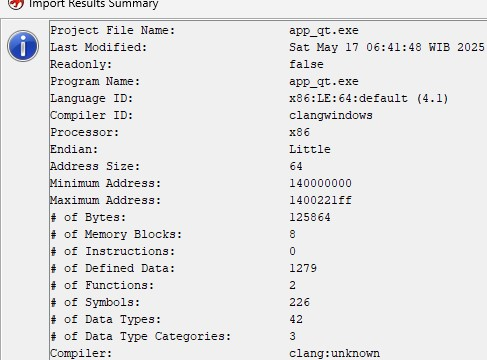
\includegraphics[width=0.9\textwidth]{assets/pics/app_qt_summary_result.jpeg} % Sesuaikan path dan ukuran
    \caption{Ringkasan Hasil Analisis Ghidra untuk \code{app\_qt.exe} (Non-Virtualized).}
    \label{fig:ghidra_summary_qt}
\end{figure}
% --- AKHIR TAMBAHAN GAMBAR GHIDRA SUMMARY QT ASLI ---

% --- TAMBAHAN GAMBAR GHIDRA SUMMARY QT VM ---
\begin{figure}[H]
    \centering
    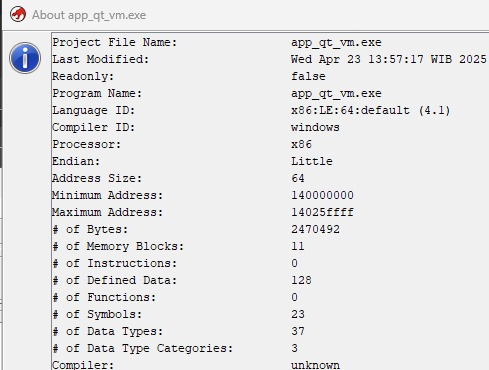
\includegraphics[width=0.9\textwidth]{assets/pics/app_qt_vm_summary_result.jpeg} % Sesuaikan path dan ukuran
    \caption{Ringkasan Hasil Analisis Ghidra untuk \code{app\_qt\_vm.exe} (Virtualized).}
    \label{fig:ghidra_summary_qt_vm}
\end{figure}
% --- AKHIR TAMBAHAN GAMBAR GHIDRA SUMMARY QT VM ---

Secara keseluruhan, data kuantitatif dari Ghidra ini memberikan bukti kuat bahwa \f{code virtualization} menggunakan VxLang secara efektif mengaburkan struktur fundamental program pada tingkat biner. Ketidakmampuan \f{disassembler/decompiler} seperti Ghidra untuk mengenali instruksi, fungsi, dan data secara signifikan meningkatkan kesulitan analisis statis. Identifikasi dan manipulasi logika autentikasi melalui pendekatan statis konvensional menjadi sangat tidak praktis dan kemungkinan besar tidak berhasil pada aplikasi yang telah divirtualisasi dengan VxLang.

\subsection{Analisis Dinamis}
Analisis dinamis dilakukan dengan menjalankan aplikasi di bawah \f{debugger} x64dbg untuk mengamati perilaku saat \f{runtime}. Tujuannya adalah untuk memverifikasi temuan dari analisis statis dan memahami bagaimana aplikasi berinteraksi dengan \f{input} pengguna, khususnya dalam proses autentikasi.

\subsubsection{Analisis Aplikasi Non-Virtualized}

Untuk aplikasi non-virtualized, analisis dinamis dilakukan dengan mencari string yang relevan dengan proses autentikasi, seperti username dan password yang ditemukan pada analisis statis ("seno" dan "rahman"). \f{Breakpoint} dipasang pada lokasi di mana \f{string} ini digunakan atau dibandingkan.

Pada aplikasi \textit{app\_qt}, saat dijalankan di bawah x64dbg dan diberikan \f{input} yang salah, \f{debugger} mengarahkan eksekusi ke blok kode berikut:

\begin{listing}[H]
    \begin{minted}[linenos=false]{asm}
; ... (Kode membandingkan input password dengan "rahman" via operator==) ...
; Hasil perbandingan (boolean) mungkin disimpan di AL atau flag register

mov al, byte ptr ss:[rbp-41]  ; Ambil hasil perbandingan
test al, 1                    ; Cek apakah hasilnya true (misal: 1)

; Perhatikan bahwa logika JNE/JE mungkin berbeda tergantung optimasi compiler
; Asumsi: JNE melompat jika perbandingan GAGAL (tidak sama)

jne SHORT failure_label       ; Lompat ke blok GAGAL jika password TIDAK sama
; ... (Kode jika password BENAR) ...

jmp END_OF_AUTH

failure_label:
; ... (Kode setup untuk menampilkan "Authentication Failed" via QMessageBox) ...

lea rdx, qword ptr ds:[<"Authentication Failed">]
; ... (call ke fungsi QMessageBox) ...

\end{minted}
\caption{Snippet Assembly: Lompatan Kondisional Setelah Perbandingan Password (Dinamis, Non-Virtualized)}
\label{lst:asm_dynamic_nonvirt_snippet}
\end{listing}

Instruksi \code{test al, 1} memeriksa hasil perbandingan password. Jika password salah (misalnya, \code{al} adalah 0), instruksi \code{jne failure\_label} (Jump if Not Equal/Zero) akan dieksekusi, mengarahkan program ke blok yang menampilkan "Authentication Failed". Dalam analisis dinamis, \textit{debugger} seperti x64dbg memungkinkan \textit{patching on-the-fly}. Dengan mengubah instruksi \code{jne} menjadi \code{je} (Jump if Equal/Zero) atau \code{jmp} (lompatan tanpa syarat ke blok sukses), pemeriksaan password dapat dilewati secara efektif saat \textit{runtime}. Konteks assembly yang lebih lengkap dari sesi debugging ini dapat dilihat di Lampiran \ref{app:kode_asm} (Kode \ref{lst:asm_dynamic_nonvirt_full}).

Sama seperti pada analisis statis, celah keamanan dapat dieksploitasi dengan memodifikasi alur eksekusi. Dalam x64dbg, instruksi `jne` dapat diubah menjadi `je` (Jump if Equal) secara langsung pada saat \f{runtime}. Dengan melakukan perubahan ini, program akan melompat ke bagian yang seharusnya dijalankan hanya jika autentikasi berhasil, meskipun \f{input} yang diberikan salah. Operasi negasi ini secara efektif melewati pemeriksaan autentikasi.

\subsubsection{Analisis Aplikasi Virtualized}

Analisis dinamis pada aplikasi yang telah divirtualisasi menggunakan x64dbg menunjukkan tantangan yang serupa dengan analisis statis. Ketika mencari string seperti "Authentication Failed", \f{debugger} sering kali tidak dapat menemukannya dalam memori proses. Hal ini mengindikasikan bahwa string tersebut mungkin tidak disimpan dalam format yang jelas atau mungkin dienkripsi dan didekripsi hanya pada saat digunakan.

Selain itu, x64dbg juga menampilkan banyak operasi dengan kategori ??? yang tidak dapat di-\f{disassemble}. Hal ini mempersulit pemahaman alur eksekusi dan fungsi-fungsi yang terlibat dalam proses autentikasi.

Lebih lanjut, melacak alur eksekusi saat memasukkan username dan password menjadi sangat sulit. Berikut adalah perbandingan \f{section} kode saat menerima \f{input} pada aplikasi konsol non-virtualized dan virtualized:


\bo{Non-Virtualized:} Menampilkan panggilan standar ke fungsi I/O C++.
\begin{listing}[H]
    \begin{minted}[linenos=false]{asm}
; ...
mov rcx,qword ptr ds:[<...std::cout>]      ; Pointer ke std::cout
lea rdx,qword ptr ds:[<"Enter username: ">] ; Pointer ke string prompt
call <console. ... std::operator<< ...>    ; Panggil fungsi print (std::cout << prompt)
; ...
mov rcx,qword ptr ds:[<...std::cin>]       ; Pointer ke std::cin
lea rdx,qword ptr ss:[rbp-28]              ; Pointer ke buffer input string
call <console. ... std::operator>> ...>    ; Panggil fungsi read (std::cin >> buffer)
; ...
\end{minted}
\caption{Snippet Assembly: Operasi Input/Output Standar (Non-Virtualized)}
\label{lst:asm_dynamic_io_nonvirt_snippet}
\end{listing}

\bo{Virtualized:} Menampilkan instruksi yang diobfuskasi dan sulit dikenali oleh debugger.
\begin{listing}[H]
    \begin{minted}[linenos=false]{asm}
??? ; Operasi tidak dikenal
jmp console_vm.vxm.7FF74CD97168 ; Lompatan internal VM?
fcmovnu st(0),st(5) ; Operasi FPU tidak relevan?
xor byte ptr ds:[rsi],ah ; Operasi XOR
??? ; Operasi tidak dikenal
jmp console_vm.vxm.7FF74CD48254 ; Lompatan pendek
fstp st(0) ; Operasi FPU
\end{minted}
\caption{Snippet Assembly: Instruksi di Lokasi Input (Virtualized)}
\label{lst:asm_dynamic_io_virt_snippet}
\end{listing}

Perbandingan ini menunjukkan kontras yang jelas. Pada kode non-virtualized, panggilan ke fungsi I/O standar seperti \code{std::cout} dan \code{std::cin} mudah dikenali. Sebaliknya, pada kode yang telah divirtualisasi, instruksi assembly menjadi tidak jelas (\code{???}), diselingi dengan lompatan (\code{jmp}) dan operasi lain yang tampaknya tidak berhubungan langsung dengan I/O (\code{fcmovnu}, \code{xor}, \code{fstp}). Hal ini menyulitkan pelacakan alur eksekusi saat input dimasukkan. Lebih lanjut, observasi menunjukkan register RIP (\f{Instruction Pointer}) seringkali tampak "\f{stuck}" pada alamat tertentu dalam \textit{debugger}, mengindikasikan eksekusi kemungkinan terjadi di dalam \textit{interpreter} mesin virtual VxLang. Hal ini sangat menyulitkan untuk melacak alur eksekusi dan memahami apa yang sebenarnya terjadi di balik layar. Perilaku ini mengindikasikan bahwa VxLang menggunakan teknik virtualisasi yang kompleks, yang secara signifikan menghambat analisis dinamis menggunakan metode tradisional seperti mencari string dan memantau alur eksekusi secara langsung. Konteks assembly yang lebih lengkap untuk perbandingan ini dapat dilihat di Lampiran \ref{app:kode_asm} (Kode \ref{lst:asm_dynamic_io_comparison_full}).

\section{Analisis Performa \f{Overhead} VxLang}
Hasil dari percobaan performa overhead dan perubahan ukuran file setelah penerapan virtualisasi kode menggunakan VxLang. Percobaan ini dilakukan pada algoritma Quick Sort dan enkripsi AES-CBC-256.

\subsection{Hasil Pengujian Performa \f{Quick Sort}}
Tabel \ref{tab:quick_sort_performance} menyajikan hasil pengukuran waktu rata-rata dan standar deviasi dari algoritma Quick Sort yang dijalankan sebanyak 100 kali untuk setiap ukuran array, baik sebelum maupun sesudah virtualisasi menggunakan VxLang.

\begin{table}[htbp]
    \centering
    \caption{Hasil Pengujian Waktu Eksekusi Quick Sort (ms)}
    \label{tab:quick_sort_performance}
    \begin{tabularx}{\textwidth}{@{}|X|X|X|X|X|@{}}
    \hline
        \multirow{2}{*}{\textbf{Ukuran Array}} & \multicolumn{2}{c|}{\textbf{Tanpa Virtualisasi}} & \multicolumn{2}{c|}{\textbf{Virtualisasi}}\\
        \cline{2-5}
        & \textbf{Rata-rata Waktu (ms)} & \textbf{Standar Deviasi (ms)} & \textbf{Rata-rata Waktu (ms)} & \textbf{Standar Deviasi (ms)}\\
        \hline
        100                     & 0.01 & 0.00 & 5.15 & 0.42 \\
        \hline
        1000                    & 0.09 & 0.00 & 53.08 & 5.52 \\
        \hline
        5000                    & 0.61 & 0.09 & 300.64 & 26.13 \\
        \hline
        10000                   & 1.38 & 0.22 & 585.70 & 79.88 \\
        \hline
        50000                   & 8.45 & 0.73 & 3,434.32 & 592.92 \\
        \hline
        100000                  & 17.86 & 1.42 & 6,771.09 & 553.09 \\
        \hline
        500000                  & 106.16 & 5.61 & 29,698.73 & 3,518.63 \\
        \hline
        1000000                 & 216.59 & 9.49 & 45,186.90 & 6,198.38 \\
        \hline
    \end{tabularx}
\end{table}

\begin{figure}[htbp]
    \centering
    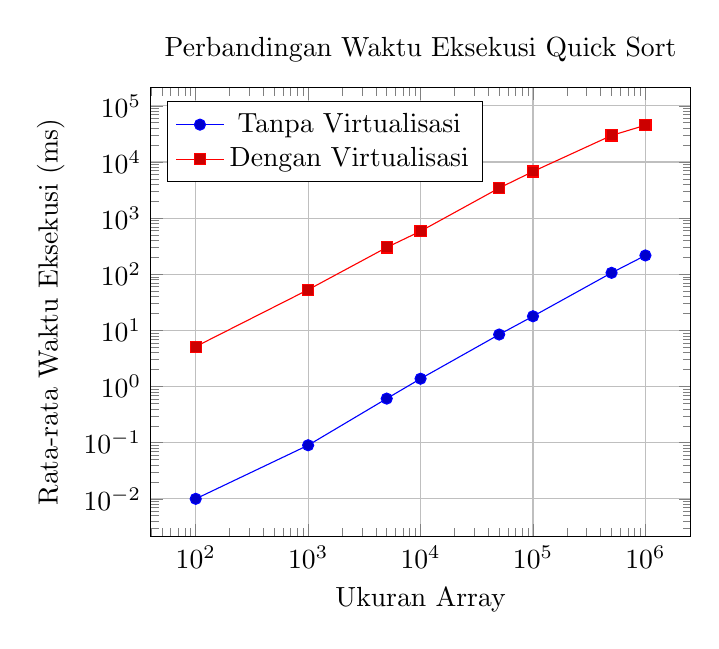
\begin{tikzpicture}
        \begin{axis}[
            xlabel={Ukuran Array},
            ylabel={Rata-rata Waktu Eksekusi (ms)},
            xmode=log,
            log basis x={10},
            ymode=log,
            log basis y={10},
            legend pos=north west,
            title={Perbandingan Waktu Eksekusi Quick Sort},
            grid=major,
        ]
        \addplot coordinates {
            (100, 0.01)
            (1000, 0.09)
            (5000, 0.61)
            (10000, 1.38)
            (50000, 8.45)
            (100000, 17.86)
            (500000, 106.16)
            (1000000, 216.59)
        };
        \addlegendentry{Tanpa Virtualisasi};

        \addplot coordinates {
            (100, 5.15)
            (1000, 53.08)
            (5000, 300.64)
            (10000, 585.70)
            (50000, 3434.32)
            (100000, 6771.09)
            (500000, 29698.73)
            (1000000, 45186.90)
        };
        \addlegendentry{Dengan Virtualisasi};
        \end{axis}
    \end{tikzpicture}
    \caption{Perbandingan Waktu Eksekusi Algoritma Quick Sort antara Versi Tanpa dan Dengan Virtualisasi VxLang.}
    \label{fig:quick_sort_performance}
\end{figure}

Berdasarkan Tabel \ref{tab:quick_sort_performance} ,terlihat adanya peningkatan waktu eksekusi yang signifikan pada algoritma Quick Sort setelah divirtualisasi menggunakan VxLang. Peningkatan ini terlihat semakin besar seiring dengan bertambahnya ukuran array. Sebagai contoh, untuk array berukuran 100, waktu eksekusi rata-rata meningkat dari 0.01 ms menjadi 5.15 ms, yang menunjukkan overhead sekitar 51400\%. Untuk array yang lebih besar seperti 1.000.000 elemen, waktu eksekusi meningkat dari 216.59 ms menjadi 45186.90 ms, dengan overhead sekitar 20860\%. Peningkatan standar deviasi juga menunjukkan bahwa waktu eksekusi menjadi lebih bervariasi setelah virtualisasi. Hal ini mengindikasikan adanya overhead yang substansial yang diperkenalkan oleh mesin virtual VxLang dalam mengeksekusi instruksi virtual dibandingkan dengan eksekusi kode native.

\subsection{Hasil Pengujian Performa Enkripsi AES-CBC-256}
Tabel \ref{tab:aes_performance} menyajikan hasil benchmarking enkripsi AES-CBC-256 dengan 1.000.000 blok data, di mana setiap blok berukuran 1024 bytes, sebelum dan sesudah virtualisasi menggunakan VxLang.

\begin{table}[htbp]
  \centering
  \caption{Hasil Pengujian Performa Enkripsi AES-CBC-256}
  \label{tab:aes_performance}
  \begin{tabular}{|l|c|c|}
    \hline
    \bo{Metrik}                                     & \bo{Tanpa Virtualisasi} & \bo{Virtualisasi} \\
    \hline
    Total Waktu Enkripsi (ms)                  & 2,722.96            & 13,193.51            \\
    \hline
    Total Waktu Dekripsi (ms)                  & 2,055.01            & 12,529.90            \\
    \hline
    Rata-rata Waktu per Blok Enkripsi (ms)     & 0.00272            & 0.01319             \\
    \hline
    Rata-rata Waktu per Blok Dekripsi (ms)     & 0.00206            & 0.01253             \\
    \hline
    \textit{Throughput} Enkripsi (MB/s)               & 358.64             & 74.02               \\
    \hline
    \textit{Throughput} Dekripsi (MB/s)               & 475.21             & 77.94               \\
    \hline
    \textit{Throughput} Gabungan (MB/s)               & 416.92             & 75.98               \\
    \hline
  \end{tabular}
\end{table}

Hasil pengujian enkripsi AES-CBC-256 menunjukkan overhead performa yang signifikan setelah penerapan VxLang. Total waktu enkripsi meningkat dari 2,722.96 ms menjadi 13,193.51 ms, yang merupakan peningkatan sekitar 384\%. Total waktu dekripsi juga mengalami peningkatan yang serupa, dari 2,055.01 ms menjadi 12,529.90 ms (sekitar 510\%). Peningkatan ini juga tercermin pada penurunan throughput (kecepatan pemrosesan data). Throughput enkripsi menurun dari 358.64 MB/s menjadi 74.02 MB/s, dan throughput dekripsi menurun dari 475.21 MB/s menjadi 77.94 MB/s. Penurunan throughput gabungan juga signifikan, dari 416.92 MB/s menjadi 75.98 MB/s. Hasil ini mengkonfirmasi bahwa virtualisasi kode dengan VxLang memperkenalkan overhead yang cukup besar pada operasi komputasi intensif seperti enkripsi.

\subsection{Hasil Pengujian Ukuran File}
Tabel \ref{tab:file_size} menyajikan ukuran file executable (dalam KB) untuk berbagai program sebelum dan sesudah virtualisasi menggunakan VxLang.

\begin{table}[htbp]
  \centering
  \caption{Hasil Pengujian Ukuran File (KB)}
  \label{tab:file_size}
  \begin{tabular}{@{}|l|c|c|@{}}
    \hline
    \multirow{2}{*}{\textbf{Program}} & \multicolumn{2}{c|}{\textbf{Ukuran File}} \\
    \cline{2-3} & \bo{Tanpa Virtualisasi} & \bo{Virtualiasi} \\
    \hline
    quick\_sort  & 119                                  & 1,951                               \\
    \hline
    encryption   & 131                                  & 1,834                               \\
    \hline
    size         & 97,802                               & 112,716                             \\
    \hline
    console      & 105                                  & 1,942                               \\
    \hline
    app\_imgui   & 1,773                                & 2,753                               \\
    \hline
    app\_qt      & 145                                  & 1,954                               \\
    \hline
  \end{tabular}
\end{table}

Hasil pengukuran ukuran file menunjukkan bahwa penerapan virtualisasi kode menggunakan VxLang secara umum meningkatkan ukuran file executable. Peningkatan ukuran file sangat signifikan untuk program-program kecil seperti quick\_sort, encryption, dan console, di mana ukurannya meningkat lebih dari sepuluh kali lipat. Untuk aplikasi GUI yang lebih besar seperti app\_imgui dan app\_qt, peningkatan ukuran file juga terlihat, meskipun persentasenya mungkin lebih kecil dibandingkan dengan program yang lebih kecil. Peningkatan ukuran file size relatif lebih kecil, namun tetap signifikan. Peningkatan ukuran ini kemungkinan disebabkan oleh penambahan interpreter mesin virtual VxLang dan bytecode yang dihasilkan ke dalam executable yang dilindungi.
